\documentclass[runningheads]{llncs}
%\documentclass{article}

\usepackage{textcomp}
\usepackage{framed}
\usepackage{amsmath}
\let\proof\relax
\let\endproof\relax
\usepackage{amsthm}
\usepackage{mathtools}
\usepackage{hyperref}
\usepackage{fnpct}
\usepackage{dirtree}
\usepackage{listings}
\lstset{language=Java,columns=flexible,numbers=left}

\makeatletter
\DeclareRobustCommand*{\lyxarrow}{%
\@ifstar
{\leavevmode\,$\triangleleft$\,\allowbreak}
{\leavevmode\,$\triangleright$\,\allowbreak}}
\makeatother

\def\bs{\char092}

\begin{document}
% This makes sure lstlisting counts without section number, just like figures
\renewcommand{\thelstlisting}{\arabic{lstlisting}}

\title{A Tutorial on Verifying \texttt{LinkedList} using KeY}
\author{{Hans-Dieter} A. Hiep\orcidID{0000-0001-9677-6644}\footnote{Corresponding author: \texttt{hdh@cwi.nl}} \and Jinting Bian \and\\
Frank S. de Boer \and Stijn de Gouw}
\authorrunning{H.A. Hiep, J. Bian, et al.}

\institute{CWI, Science Park 123, 1098 XG Amsterdam, The Netherlands\\
\email{\{hdh,j.bian,frb,stijn.de.gouw\}@cwi.nl}}

\maketitle

\begin{abstract}
This is a tutorial paper on using KeY to demonstrate formal verification of state-of-the-art, real software. We explain in sufficient detail for a beginning user of JML and KeY, the specification and verification of part of a corrected version of the \texttt{java.util.LinkedList} class of the Java Collection framework.
\end{abstract}

\keywords{KeY, Java Modeling Language, cyclic data structure, case study}

\section{Introduction}

Software libraries are the building blocks of many programs that run on the devices of many more users every day. The functioning of a system may rely for a large part on its used software libraries. A small error present in a heavily-used software library could lead to serious unwanted outcomes, such as system outages and failures. Using root cause analysis, one could find from a system failure the errors that have caused it. But root cause analysis can only applied \emph{after} a failure has happened. To prevent failures from happening in the first place, correctness is of the utmost importance. Although establishing program correctness seems to be an expensive activity, it may be worthwhile for critical software libraries, such the standard library that all programs rely on.

This tutorial intends to show how we take an existing Java program that is part of the Java standard library, and study it closely to increase our understanding of it. If we are only interested in showing the presence of an issue with the program, e.g.~that it lacks certain functionality, it suffices to show an example run which behaves unexpectedly. But to reach the conclusion that no unexpected behavior ever results from running the program, first requires a precise specification of what behavior one expects, and further requires a convincing argument that all possible executions of the program exhibit that behavior.

We take a formal approach to both specification and reasoning about programs, allowing us to increase the reliability of our reached conclusions. In particular, the specifications we write are expressed in the Java Modeling Language (JML), and our reasoning is tool-supported and partially automated by KeY. To the best of the authors' knowledge, KeY is the only tool that supports enough features of the Java programming language for reasoning about realistic programs, of which its run-time behavior crucially depends on the presence of such features, such as: dynamic object creation, exception handling, integer arithmetic with overflow, \texttt{for} and \texttt{foreach} loops with early returns, nested classes (both static and non-static), inheritance, polymorphism, erased generics, etc.

As a demonstration of applying KeY to real software, we will focus on Java's \texttt{LinkedList} class for two reasons. First, a (doubly-)linked list is a well-known basic data structure for storing and maintaining unbounded data, and has many applications: for example, in Java's secure sockets implementation. Second, it has turned out that there is a 20-year-old bug lurking in its program, that might lead to in-depth security issues on large memory systems, caused by the overflow of a field that caches the length of the list \cite{hiep2019verifying}. Our specification and verification effort will be aimed at establishing the absence of this bug from a repaired program.

In this tutorial, we see how to set-up a project and configure the KeY tool, and outline the general workflow that we follow (Section~\ref{sec:setup}). We then study the source code of the \texttt{LinkedList}, and get an intuitive grasp of its essential structure: how the various instances of this class look like, and how some essential methods operate on these instances (Section~\ref{sec:linkedlist}). A basic introduction to the KeY system is given, on which the rest of the tutorial builds (Section~\ref{sec:background}).

To keep this presentation reasonably short, we focus only on the methods \texttt{add} and \texttt{remove}. We shall formulate, based on previous intuition, a \emph{class invariant} in JML that expresses a property that is true of every instance and must remain true after executing our methods (Section~\ref{sec:class-invariant}). We use the invariant in formulating a \emph{method contract} for the \texttt{add} method that describes its expected behavior and we verify that its implementation is correct (Section~\ref{sec:add}).

The difficulty level increases after we specify the \texttt{remove} method (Section~\ref{sec:remove}), as its verification requires more work than before. A lemma is needed, one that follows from the invariant (Section~\ref{sec:acyclicity}). We study the deeper methods that \texttt{remove} depends on first (Section~\ref{sec:unlinking}), and use \emph{loop invariants} to prove the correctness of \texttt{remove} later (Section~\ref{sec:loop-invariant}). We conclude with some methods of \texttt{LinkedList} left as exercise to the reader (Section~\ref{sec:conclusion}): finding their specifications and proving them correct is not trivial, but done in a similar way.

This tutorial is mainly based on the results as described in a paper \cite{hiep2019verifying} by the same authors, yet to appear. That paper provides more details on the specification and verification effort of the linked list class as a whole, including multiple test cases which trigger the overflow error, and the future verification challenges.

\section{Set-up}\label{sec:setup}

\begin{table}[]
\dirtree{%
.1 linkedlist-tutorial.
.2 key-2.6.3.zip.
.2 LinkedList.key.
.2 src.
.3 java.
.4 util.
.5 LinkedList.java.
.5 LinkedList.solution.
.2 jre.
.3 java.
.4 ....
.2 proof.
.3 ....
}
\medskip
    \caption{Directory structure of project files. The \texttt{src} directory contains the Java classes we want to specify and verify. The \texttt{jre} directory contains stub files, with specifications of unrelated classes. The \texttt{LinkedList.solution} file is the source file we end up with after following this tutorial. The \texttt{proof} directory contains the completed proofs of the solution.}
    \label{tab:directory-structure}
\end{table}

First we will set-up the project files needed to use KeY. The project files are available on-line: these can be downloaded and include the KeY software version that we use. ??? After unpacking the project files, we end up with the directory structure of Table~\ref{tab:directory-structure}.

The original source file of \texttt{LinkedList.java} was obtained from OpenJDK version \texttt{jdk8-b132}. The original has been pre-processed: generic class parameters are removed, and all methods and nested classes irrelevant to this tutorial are removed. Both the removal of generics and the stub files in the \texttt{jre} folder were generated automatically, using the Eclipse extensions for KeY. Repeating these steps is not necessary here.

Over the course of next sections, we will insert code into the linked list: annotations to formally specify its behavior, and helper methods for presenting intermediary lemmas. The annotations are usual Java comments, and thus ignored when the file is read by a Java compiler. The helper methods introduce slight performance overhead (of calling a method that performs no operations, and immediately returning from it); it is immediately clear that these do not change the original behavior of the program.

\subsection{KeY settings}

\begin{table}[]
    \begin{tabular}{l@{\hskip6pt}|@{\hskip6pt}l}
    \textbf{JavaCard} & \textbf{Off} \\
    Strings & On \\
    Assertions & Safe \\
    BigInt & On \\
    Initialization & Disable static initialization \\
    \textbf{Int Rules} & \textbf{Java semantics} \\
    Integer Simplification Rules & Full \\
    Join Generate Is Weakening & Off \\
    Model Fields & Treat as axiom \\
    \textbf{More Sequence Rules} & \textbf{On} \\
    Permissions & Off \\
    Program Rules & Java \\
    Reach & On \\
    Runtime Exceptions & Ban \\
    Sequences & On \\
    Well-definedness Checks & Off \\
    Well-definedness Operator & L
    \end{tabular}
    \medskip
    \caption{The taclet options we use. The boldface options are changed from the default. The JavaCard setting is changed from On to Off, the Int Rules settings is changed from ignoring overflow to Java semantics, and the More Sequence Rules is changed from Off to On.}
    \label{tab:taclet-options}
\end{table}

To produce proofs in KeY, the first step is to set-up KeY's taclet base to make use of particular groups of rules that correctly model Java's integer overflow semantics. This has to be done only once, as these taclet settings are stored per computer user.

Sometimes, KeY overwrites or corrupts these settings if different versions are used. To ensure KeY starts in a fresh state, one can remove the \texttt{.key} directory from the user's home director, and clean out preferences from the \texttt{.java/.userPrefs} directory by deleting the \texttt{de/uka/ilkd/key} hierarchy containing \texttt{prefs.xml} files\footnote{On Windows, the preferences are instead stored in the Windows Registry. Use the \texttt{regedit} tool and clean out under \texttt{HKEY\_CURRENT\_USER\bs Software\bs JavaSoft\bs Prefs} or \texttt{HKEY\_CURRENT\_USER\bs Software\bs Wow6432Node\bs JavaSoft\bs Prefs} the same hierarchy. On Mac OS, open a terminal, change directory to \texttt{\textasciitilde/Library/Preferences} and delete \texttt{de.uka.ilkd.plist}}.

Now start up KeY, and the example selection screen appears (if not, selecting File\lyxarrow Load Example opens the same screen). Load any example, to enter proof mode. Select Options\lyxarrow Taclet Options, and configure the options as in Table~\ref{tab:taclet-options}.

After setting these taclet options, they become effective after loading the next problem. We do that now: the main proof file \texttt{LinkedList.key} can be loaded, and a contract selection window opens up, showing a class hierarchy and its methods. A method is not shown when no specifications for it are written. After following the examples below, more method contracts can be selected in this window.

\subsection{Workflow}

\begin{figure}
    \centering
    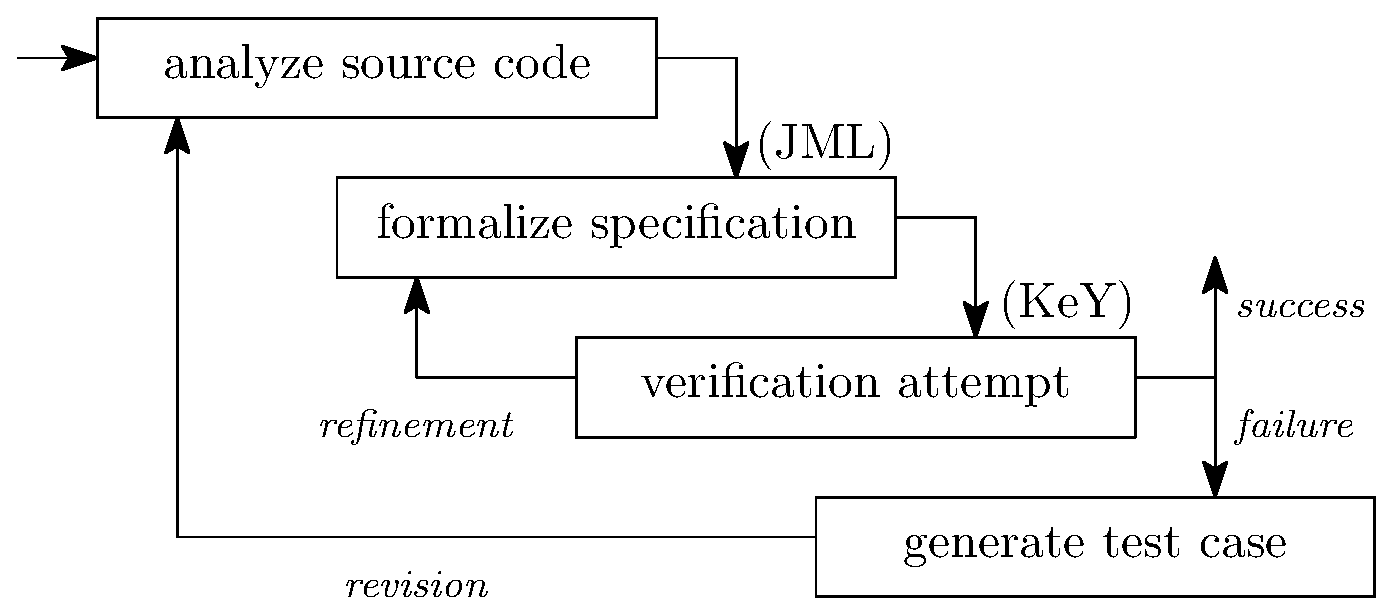
\includegraphics[width=272pt]{figures/workflow.eps}
    \caption{The workflow for our verification process.}
    \label{fig:workflow}
\end{figure}

We start by analyzing the source code, to gain an intuitive understanding of the linked list class. From that we formalize a specification (in JML). After formalizing the specification, we attempt to verify its methods (using KeY). Our attempt could fail because the specification is not sufficiently detailed: we refine the specification. Another reason for failure to verify is that the source code contains an error: in this case, we can demonstrate the unexpected behavior by writing a test case. The test case then shows there is a run in which the linked list behaves unexpectedly. This leads to a revision of the source code to fix the error. Now, the specification has to be reviewed and the verification attempt can continue. We are successful once the verification attempt is completed with a formal proof. This workflow is depicted as a flow diagram in Fig.~\ref{fig:workflow}.

\section{\texttt{java.util.LinkedList}}\label{sec:linkedlist}

In this section we walk through part of the source code of the \texttt{LinkedList} class. Over the course of this tutorial, we will edit this file to add annotations at the appropriate places.

\lstinputlisting[linerange=1-10,frame=single,caption={The \texttt{LinkedList} class fields and constructor.},captionpos=b,label={lst:linkedlist}]{src/java/util/LinkedList.java}

The \texttt{LinkedList} class has three attributes: a \texttt{size} field, which stores a cached number of elements in the list, and two
fields that store a reference to the first and last \texttt{Node} (see Listing~\ref{lst:linkedlist}).

The linked list fields are declared transient and package private. The transient flag is used to control serialization and deserialization: but that is out of scope of our verification effort. The reason the fields are declared package private seem to prevent generating accessor methods by the Java compiler. However, in practice, the fields are treated as they were private.

The \texttt{Node} class is defined as a private static nested class to represent the containers of items stored in the list (see Listing~\ref{lst:linkedlist-node}). A static nested private class behaves like a top-level class, except that it is not visible outside the enclosing class. The nodes are doubly-linked, that is, each node is connected to its preceding node (through field \texttt{prev}) and succeeding node (through field \texttt{next}). These fields contain \texttt{null} in case no preceding or succeeding node exists. The data itself is contained in the \texttt{item} field of a node.

\lstinputlisting[firstnumber=65,linerange=65-75,frame=single,caption={The \texttt{Node} nested class fields and constructor.},captionpos=b,label={lst:linkedlist-node}]{src/java/util/LinkedList.java}


Constructor, add method, remove method

\subsection{Expected behavior}
Pictures of instances

Pictures of adding

Pictures of removing

\subsection{Bugfix}
Short description of bug

Short fix to problem (checkSize)

\section{Background}\label{sec:background}

The \emph{KeY system} consists of three main components: a multi-sorted classical first-order sequent calculus with a large rule set, a translator of annotated Java programs into proof obligations, and an interactive tool for creating proofs.

\paragraph{Dynamic logic}
The logic underlying KeY is \emph{JavaDL}, a program logic that directly incorporates Java program fragments.
The program logic is a multi-modal logic: $\langle P\rangle\varphi$ expresses that executing the program fragment $P$ definitely terminates and $\varphi$ holds in the final state; and $[P]\varphi$ expresses \emph{if} the program fragment $P$ terminates, \emph{then} $\varphi$ holds in the final state. The formula $\varphi\to\langle P\rangle\psi$ expresses that if $\varphi$ holds in the initial state, then execution of $P$ terminates in a state for which $\psi$ holds.  See Chapter 3 of~\cite{ahrendt2016deductive} for more detail of JavaDL's syntax and semantics.

The program logic distinguishes \emph{program variables} from \emph{logical variables}: the value of a program variable can be changed over the course of executing a program, whereas a logical variable always has the same value. As logical variables can never be modified by a program fragment, they are used as so-called \emph{freeze variables}.

The proof system that KeY uses to establish validity of formulas is given as a sequent calculus. A sequent $\varphi_1,\ldots,\varphi_n \Rightarrow \psi_1,\ldots,\psi_m$ consists of $n$ antecendents and $m$ consequents, all formulas of JavaDL, with the usual interpretation: $\varphi_1,\ldots,\varphi_n \Rightarrow \psi_1,\ldots,\psi_m$ means that if all $\varphi_i$ on the left are true, then at least one $\psi_j$ on the right is true. Next to the rules for classical first-order logic, the proof system also consists of a large number of other rules. The large rule set is given by means of lightweight tactics (called taclets \cite{beckert2004taclets}) that perform modifications on the sequent one is proving: e.g.~spawn new branches in the proof tree, substitute variables, rewrite terms, or close a branch. There are approximately 1750 rules that implement Java program semantics and allow for symbolic execution, and implement the theories of many sorts: integers, sequences, heaps, location sets, and others.

Of particular interest to us are rules concerning \emph{updates} and \emph{heaps}. There are rules that transform modalities with program fragments into so-called update modalities. Updates always terminate and they assign JavaDL terms to program variables. As such, updates cannot assign program variables to side-effectful expressions. Given a formula $\varphi$, then $\{\mathtt{x}_1\coloneqq t_1||\ldots||\mathtt{x}_n\coloneqq t_n\}\varphi$ is a formula where in parallel $\mathtt{x}_i$ are updated to $t_i$.

\paragraph{Data types}
There is a hidden and implicit program variable in JavaDL that is the \texttt{heap} of heap sort. The heap is used to model the storage of objects, that is, the value of fields associated to object references. From a practical perspective, updates of program variables other than the heap can be thought of as stack variables. Such program variables can \emph{refer} to objects on the heap. Heap updates are tracked by updating the \texttt{heap} program variable. Heap updates and program variable updates easily form complex expressions, where both kinds of updates can be intertwined: we do not show heap update expressions here, but see Section 2.4.3 and Section 6.4 of \cite{ahrendt2016deductive}.

Next to the built-in sorts of integers, sequences, heaps, and location sets, are Java types. Each Java type has its own sort in JavaDL that models (infinitely many) references to objects, including the \texttt{\textbf{null}} reference. References can be explicitly coerced between sorts, to model subtypes: e.g. every reference can be coerced to a reference of sort \texttt{Object}. A heap assigns values to the fields of a non-null reference.
Object references are global, but the creation status of each object is a special Boolean field \texttt{<created>} local to each heap. An object becomes created in some heap by taking a fresh reference, that has no value yet assigned to its creation field in that heap, and setting that field to \texttt{\textbf{true}}. Fields can only be assigned to non-null object references for which their created field is true. A heap is \emph{well-formed} if a finite number of references have \texttt{<created>} set to true.

\paragraph{JML}
\begin{figure}
   \centering
   \includegraphics{figures/method_heap.eps}
   \caption{Heaps are `threaded' through method calls. In heap $H_1$ the program fragment $P$ is executed, resulting in heap $H_2$. Either a contract for method \texttt{m()} is employed, which relates the before heap $H_b$ to some heap after the method call $H_a$; or, the method body is unfolded by wrapping it in a method frame that resolves overshadowing of program variables. In both cases, to call the method, heap $H_b$ is equal to $H_2$ and heap $H_a$ is equal to $H_4$. Then the program fragment $P'$ that occurs after the method call is executed using the heap returned by the method.}
   \label{fig:method_heap}
\end{figure}

An important aspect of Java programs are method calls. There are three main issues: calling a method may introduce new program variables that overshadow older program variables, calling a method may change the heap, and it is possible to call a method on an object for which its exact type is only known at run-time.

To solve the issue of overshadowing older program variables, KeY uses \emph{method frames}; before a method frame is created, it is ensured that old program variables and new program variables do not collide by renaming the program variables of a method body. Since the \texttt{\textbf{this}} keyword cannot be renamed, the method frame provides a context in which program fragments evaluates \texttt{\textbf{this}} references; it also tracks where the method return value must be placed. The heap supplied to the method call is the heap as it was after the statements that occurred before the method call, and statements following a method call are performed using the heap as it is after the method call completes: there are rules for `threading' the heap through a method call, see Figure \ref{fig:method_heap}. There are roughly two ways of treating method calls: unfolding their method body wrapped in a method frame, or using its method contract.

Method contracts and general annotations of Java programs are specified in terms of a subset of the Java Modeling Language (JML)~\cite{leavens2013jml} but with KeY-specific extensions, see \cite{huisman2014jml} or Chapter 7 of~\cite{ahrendt2016deductive}. This allows the use of KeY for post-hoc verification: after a program has been developed and validated, classes and their members are annotated. In particular, each method is annotated by a contract that specifies pre- and post-conditions. In this approach, methods are the central point of our verification effort. Its annotations determine corresponding correctness formulas in JavaDL: if they are verified, then the corresponding method is correct with respect to its method contract. Consequently, method contracts can be reused in other proofs involving program fragments that call such method.

Other than method contracts, JML also allows annotations of ghost fields, model fields and model methods. Ghost fields are virtual fields that become part of the modelled state of an object on the heap, but are never present when actually executing a Java program. Like normal fields, the value of ghost fields are assigned a default value at object initialization, and can be explicitly changed by JML \texttt{set} annotations. These annotations occur anywhere in method bodies where otherwise a normal statement can be expected. Model fields are introduced as function symbols, and several axioms are added that allow the definition of model fields to be substituted during proof. An example model field is a \emph{class invariant}, which is implicitly assumed to hold of the state of an object between method invocations. More general than model fields are model methods: every model field is implemented as a specific model method. Other annotations, such as loop invariants, are also added to the method body: these are automatically applied by KeY's symbolic execution.

Java programs annotated with JML are entered into the KeY system and the verification of their correctness formulas begins, by generating one or more \emph{proof obligations} for each correctness formula. Using the interactive tool, a proof tree is constructed by applying rules until the branches of the tree are closed. Each rule application may result in zero or more branches: in the case of multiple branches, every branch needs to be closed. The tool also provides automation, that automatically applies proof rules using heuristics. This speeds up the verification effort considerably. Finally, after all proof obligations appear as the conclusion of a closed proof tree, the verification effort is done. The proof trees can be stored in a file and reloaded and inspected later.

\section{Class invariant}\label{sec:class-invariant}

Each linked list consists of a sequence of nodes. Sequences are finite, indexing of sequences starts at zero, and we write $\sigma[i]$ to mean the $i$th element of some sequence $\sigma$. A \emph{chain} is a sequence $\sigma$ of nodes of length $n>0$ such that: the \texttt{prev} reference of the first node $\sigma[0]$ is \texttt{null}, the \texttt{next} reference of the last node $\sigma[n-1]$ is \texttt{null}, the \texttt{prev} reference of node $\sigma[i]$ is node $\sigma[i-1]$ for every index $0<i<n$, and the \texttt{next} reference of node $\sigma[i]$ is node $\sigma[i+1]$ for every index $0\leq i < n-1$. The \texttt{first} and \texttt{last} references of a linked list are either both \texttt{null} to represent the \emph{empty} linked list, or there is some chain $\sigma$ between the \texttt{first} and \texttt{last} node, viz.~$\sigma[0]=\mathtt{first}$ and $\sigma[n-1]=\mathtt{last}$. Figure \ref{fig:linkedlist} shows example instances.
Also see standard literature such as Knuth's \cite[Section 2.2.5]{knuth1997art}.

\begin{figure}[t]
  \centering
  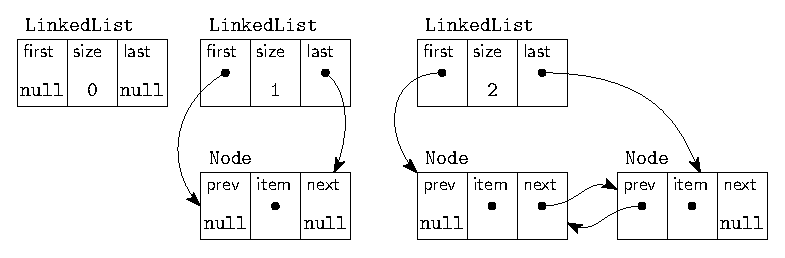
\includegraphics[scale=0.75]{figures/linkedlist1.eps}
  \caption{Three example linked lists: empty, with a chain of one node, and with a chain of two nodes. Items themselves are not shown.}
  \label{fig:linkedlist}
\end{figure}

\subsection{Cached vs. real size}
\subsection{Ghost node list}
\subsection{Reference structure}

\section{The constructor}\label{sec:constructor}

Select the constructor from the method selection screen.

Strategy we use:
max. rule applications 1000
stop at: default
proof splitting: delayed
loop treatment: invariant
block treatment: contract
method treatment: contract
dependency contract: on
query treatment: off
expand local queries: on
arithmetic treatment: basic
quantifier treatment: no splits with progs
class axiom rule: off
auto induction: off
user-defined taclets: all off

Right click on the proof tree root node, and select "Hide non-interactive proofsteps" and "Hide closed subtrees".

Right click on open goal from the Proof window, select strategy macros, auto pilot, finish symbolic execution.

Two branches remain: a normal execution (self != null), and a null reference (self = null). Right click on the proof tree, close provable goals below. Now one of the two branches is closed (the null reference branch). In the remaining goal, select the whole sequent, strategy macros, simplification, update simplification.

In one of the consequents, we see a formula that is a conjunction of the post-condition of the constructor (that the node list is empty, \texttt{self.nodeList@heap[...] = seqEmpty}), the class invariant (\texttt{self.<inv>}), and that no exception occurred (\texttt{null = null}). Right click the formula and select strategy macros, propositional, propositional expansion (with splits). This generates three open goals, one for each conjunct.

Right click the proof root, select strategy macros, close provable goals below. Only a single goal remains: that of the invariant.

Click the invariant and select the Class invariant rule. The invariant is expanded into a large conjunction, that we specified as class invariant, but with the updated heap distributed in. Select the resulting conjunction, and perform propositional expansion with splits. This generates 23 goals. Now select a node in the proof tree above these and close provable goals. All of them are automatically closed.

Nodes: 1195
Branches: 29
Interactive steps: 1

Note that this method can also be proven correct fully automatically.

\section{The \texttt{add} method}\label{sec:add}

Open the proof manager (File, Proof Manager) and select checkSize. There are two contracts: we start with normal behavior.

Select the open goal in the proof window, auto pilot, finish symbolic execution. It generates two goals: if x is true and if x is false. Here x is the condition whether the maximum size of the list has been reached.

In the first branch, x is true, perform update simplification only on the whole sequent\footnote{Bug in key: must do on whole sequent}. There is now a conjunction in the consequent, and we do propositiobnal expansion with splits on it. The remaining goal can be closed automatically.

In the second branch, x is false, also perform update simplification only on the whole sequent. There is a formula in the consequent with three conjuncts: the class invariant, that no exception is thrown, and that no heap modification has happened. Apply propositional expansion with split on the formula: it generates two goals, that can be closed automatically by selecting close provable goals.

Nodes: 201
Branches: 8
Interactive steps: 0

Note that this method can also be proven correct fully automatically.

---

Open proof manager (Ctrl+M), select checkSize and the exception behavior contract. Apply strategy (green arrow button), and see that it can be closed fully automatically.

Nodes: 249
Branches: 4
Interactive steps: 0

---

Open proof manager, select linkLast and the normal behavior contract.

Select the open goal, and finish symbolic execution. It generates 8 goals. Select the root node in the proof tree, closing provable goals below. Only two goals remain: if x true and if x false, this corresponds to whether the last field was null (x true) or not (x false).

In the first branch, x is true, we do update simplification only on the whole sequent. We first hide a formula in the antecedent (\texttt{e = null | e.<created> = true}), because that might generate too many branches, while the information it contains is not needed in the rest of the proof. Right click that formula, and select hide\_left. Now select the whole sequent and select propositional expansion with split: it generates 4 goals. Select close provable goals above them in the proof tree. Only one goal remains: that is to establish the class invariant after the method. Use the class invariant rule on the formula in the consequent: it generates a large conjunction. Use propositional expansion with split on the resulting goal; it generates 23 goals. Select close provable goals above them in the proof tree: all of the 23 goals can be closed automatically.

In the second branch, x is false, is the same recepi as in the first branch. However, this time, not all 23 goals can be closed automatically: we remain with two open goals. The two goals correspond to the two properties that establish the links between the nodes.

In the first remaining open goal (it is a complex rendition of nodeList[i].prev = nodeList[i - 1]), we apply the allRight rule and the impRight rule. This adds the left-hand side of the implication to the antecent of the sequent. Click on the self.nodeList@heap[...] sub expression and select "Apply rules automatically here". It generates a number of (not very intelligable) goals; these can all be closed automatically.

In the second remaining open goal (it is a complex rendition of nodeList[i].next = nodeList[i + 1]), is fully analogous as the previous remaining open goal. However, also this time, not all goals automatically close. We remain with one open goal: (** intuitive comment the proof situation is as follows. We assume that there is an index i, such that nodeList[i] = last. But also, we assume that index i < nodeList.length - 1. But we know from the invariant, that i = nodeList.length - 1 for the last node. From this, we derive the contradiction. **). We expand the class invariant; propositional expansion with split. The empty branch can close automatically. We now also have in the antecedent that nodeList[nodeList.length - 1] = last. From the invariant, by quantifier instantiation (rule allLeft), we know that nodeList[i].next = nodeList[i + 1]. We perform impLeft on the resulting formula, generating two goals. One closes automatically, because it is a simple bounds check. Now, technically, we compare the two formulas: nodeList[i] = last, and the one resulting from the quantifier instantation: (Node)(nodeList[i]).next. The latter has a superflous cast: we remove it by applying the castedGetAny rule. Now we can equationally rewrite, by applying the rule applyEq on the resultant subformula. We then obtain self.last.next = (Node)nodeList[i + 1]. But we also know self.last.next = null; so by showing that (Node)nodeList[i + 1] != null, we are done. But that (Node)nodeList[i + 1] != null follows from the class invariant: nodeList[i + 1] instanceof Node. We apply quantifier instantiation (rule allLeft) with the term i + 1. Again, we apply impLeft and close one goal which is a simple bounds check. From the remaining part, we split the conjunction and narrow type on the formula that expresses nodeList[i + 1] != null. We apply the rule notLeft, and the goal can be closed after symmetry of equality.

Nodes: 10,279
Branches: 127
Interactive steps: 21

---

Open proof manager, select add, normal behavior.

Select goal, and perform symbolic execution, and close provable goals. We have one remaining goal: it still contains a modality with a Java program fragment. We manually execute it by performing the rules: methodCallReturn, assignment, methodCallEmpty, tryEmpty, emptyModality. On the remaining whole sequent, apply update simplification only. Split the conjunction in the consequent: this generates 4 goals. We then close provable goals automatically, resulting in a complete proof.

Nodes: 2,179
Branches: 9
Interactive steps: 5

---

Open proof manager, select add, exceptional behavior. Apply strategy (green arrow button), and see that it can be closed fully automatically.

Nodes: 217
Branches: 6
Interactive steps: 0

\section{The \texttt{remove} method}\label{sec:remove}
\section{Acyclicity}\label{sec:acyclicity}

Open proof manager, select lemma\_acycliic. Finish symbolic execution. On the whole sequent, update simplification only. Propositional extension with split on consequent. Close provable goals on root. One remaining goal: the lemma we want to prove.

Introduce quantifier (allRight). Propositional expansion without split. Introduce quantifier (allRight). Not right.

Current goal:
nodeList[j] = nodeList[i], ..., self.<inv> => i <= -1, i >= nodeList.length - 1, j <= i, j >= nodeList.length

Cut formula:
(forall int k; j <= k & k < nodeList.length -> self.nodeList[k] = self.nodeList[k - (j - i)])

Two branches. First branch, we assume the cut formula is true. Eliminate quantifier, allLeft, for (nodeList.length - 1). Apply impLeft. Two cases. First is bounds check, closes automatically. Second case: unfold invariant, propositional extension with split. Two cases: empty, non-empty. The empty case closes automatically. (** We reach contradiction. **) For self.last = nodeList[nodeList.length - 1], apply rules automatically, but rewrite the size back to length. We also rewrite with self.last.next = null. Instantiate quantifier (forall i nodeList[i].next = nodeList[i+1]) for term (nodeList.length - 1 - (j - i)). Apply impLeft: two cases, the first is bounds check which closes automatically. Instantiate quantifier (forall i, nodeList[i] != null) for term (nodeList.length - (j - i)). Apply impLeft: two cases, the first case is bounds check which closes automatically.

We now have: nodeList[nodeList.length - (j - i)] != null, but also nodeList[nodeList.length - (j - i)] = null (from last.next = null). Narrow type the former, equational rewriting. Closing.

\section{Unlinking}\label{sec:unlinking}
\section{Loop invariants}\label{sec:loop-invariant}
\section{Conclusion}\label{sec:conclusion}

\bibliographystyle{splncs04}
\bibliography{base}

\end{document}
\endinput
